\documentclass{article}

\usepackage{amsmath, amsthm, amssymb, amsfonts}
\usepackage{thmtools}
\usepackage{graphicx}
\usepackage{setspace}
\usepackage{geometry}
\usepackage{float}
\usepackage{hyperref}
\usepackage[utf8]{inputenc}
\usepackage[english]{babel}
\usepackage{framed}
\usepackage[dvipsnames]{xcolor}
\usepackage{tcolorbox}

\graphicspath{ {./images/} }

\colorlet{LightGray}{White!90!Periwinkle}
\colorlet{LightOrange}{Orange!15}
\colorlet{LightGreen}{Green!15}

\newcommand{\HRule}[1]{\rule{\linewidth}{#1}}

\declaretheoremstyle[name=Ejemplo,]{thmsty}
\declaretheorem[style=thmsty,numberwithin=subsection]{ejemplo}
\tcolorboxenvironment{ejemplo}{colback=LightGray}

\declaretheoremstyle[name=Theorem,]{thmsty}
\declaretheorem[style=thmsty,numberwithin=section]{theorem}
\tcolorboxenvironment{theorem}{colback=LightGray}

\declaretheoremstyle[name=Proposition,]{prosty}
\declaretheorem[style=prosty,numberlike=theorem]{proposition}
\tcolorboxenvironment{proposition}{colback=LightOrange}

\declaretheoremstyle[name=Principle,]{prcpsty}
\declaretheorem[style=prcpsty,numberlike=theorem]{principle}
\tcolorboxenvironment{principle}{colback=LightGreen}

\setstretch{1.2}
\geometry{
    textheight=9in,
    textwidth=5.5in,
    top=1in,
    headheight=12pt,
    headsep=25pt,
    footskip=30pt
}

% ------------------------------------------------------------------------------

\begin{document}

% ------------------------------------------------------------------------------
% Cover Page and ToC
% ------------------------------------------------------------------------------

\title{ \normalsize \textsc{}
		\\ [2.0cm]
		\HRule{1.5pt} \\
		\LARGE \textbf{\uppercase{Apunte Olimpiadas Ñandu}
		\HRule{2.0pt} \\ [0.6cm] \vspace*{10\baselineskip}}
		}
\date{}
\author{\textbf{Autor} \\ 
		Ignacio Cuevas \\
		Cordoba, Argentina \\
		2023}

\maketitle
\newpage

\tableofcontents
\newpage

\section{Introduccion a las Competencias}

\subparagraph*{}
\begin{small}
En este apunte vamos a estudiar los diferentes tipos de problemas que nos podemos encontrar en la Olimpiada de Matematicas Ñandu (Tercer nivel) y vamos a aprender algunas herramientas que nos seran util para resolver cada uno de los problemas.
\end{small}

\newpage

\section{La Competencia}

\subparagraph*{}
\begin{small}
La competencia consta de 3 ejercicios:
\begin{enumerate}
	\item El primer ejercicio de Algebra
	\item El segundo de Geometria
	\item Y el tercero de Conteo
\end{enumerate}
Ahora pasaremos a explicar cada uno de ellos.
\end{small}

\subsection{Algebra}
\begin{small}
En este primer tipo de ejercicios nos vamos a encontrar problemas donde nos presentan un tipo de objeto (por ejemplo, verduras), y ciertos valores de ellos (por ejemplo, su precio), ya sea el objeto individual o sumas de varios. Veamos un ejemplo para que quede mas claro.
\\
\end{small}

\begin{ejemplo}
En las bolsas A, B y C hay en total 200 caramelos. En la bolsa B hay 20 más que
en la A, en la bolsa C hay 61 más que en la B. ¿Cuántos caramelos hay en la bolsa C?
\end{ejemplo}

\begin{ejemplo}
En el colegio hay 1360 alumnos inscriptos. De los alumnos inscriptos, $\frac{3}{5}$ se anotaron en el turno mañana. De los alumnos del turno mañana, $\frac{1}{4}$ van al jardín, $\frac{2}{3}$ van a la primaria y los demás van a la secundaria. ¿Cuántos alumnos van a la secundaria en el turno mañana?
\end{ejemplo}

\subsection{Geometria}
\begin{small}
Este segundo ejercicio es de geometria, es decir, nos vamos a encontrar con un ejercicios que involucran figuras, lados, angulos.
El dibujo puede estar dado en el ejercicio, o pueden dar las caracteristicas para que uno lo grafique. Estos dibujos muchas veces tienen puntos clave representados con letras.
Los datos que nos dan pueden ser las medidas de algunos lados, angulos, perimetros, areas, etc.
\\
\end{small}

\begin{ejemplo}
ABCD es un rectángulo,
AB = 3BC;
M es punto medio de AB;
N es punto medio de AD;
P es punto medio de CD;
O es el punto medio del segmento MP.
El perímetro de AMPD es de 80cm.
¿Cuál es el perímetro de AMON?
¿Cuál es el área de BCPO?

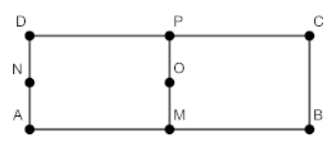
\includegraphics[scale=0.6]{geometry-example-1}
\end{ejemplo}

\begin{ejemplo}
En la figura:
ABC es un triángulo equilátero,
EFGH es un rectángulo,
CDE es un triángulo rectángulo,
F es punto medio de AB,
G es punto medio de BC,
DE = AB,
Perímetro de ABC = 96cm.
¿Cuál es el área de EFGH?
¿Cuál es el perímetro de CDFG?
¿Cuál es el área de ABCD?
¿Cuál es el área de CDG?

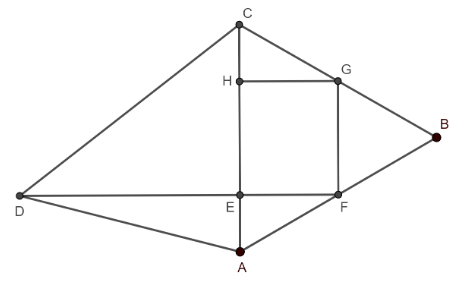
\includegraphics[scale=0.6]{geometry-example-2}
\end{ejemplo}

\subsection{Conteo}
\begin{small}
Este ultimo ejercicio, como bien dice su nombre, tenemos que contar cosas. Pueden ser numeros en un cierto rango que cumplen ciertas propiedades, formas de hacer determinada cosa, u otras cosas. Como datos nos van a dar el problema y sus restricciones.
\\
\end{small}

\begin{ejemplo}
Luis come, en total, 5 chocolatines en la semana, de lunes a viernes.
Puede comer 2 chocolatines, 1 chocolatín o ningún chocolatín en el mismo día.
En esta tabla anota cuántos chocolatines come cada día.
¿De cuántas maneras distintas puede completar la tabla?
Explica cómo las contaste.
\end{ejemplo}

\begin{ejemplo}
Aníbal y Beto están en el equipo de pingpong.
Martín, Nicolás, Oscar y Pablo están en el equipo de tenis.
Ramón, Santiago y Tomás están en el equipo de natación.
Entre estos deportistas deben elegir un grupo de 5 para hacer un viaje.
Si en el grupo debe haber por lo menos un representante de cada deporte,
¿de cuántas maneras distintas puede hacerse la elección?
Explica cómo las contaste.
\end{ejemplo}

\newpage

\section{Algebra}
\begin{small}
En este primer modulo vamos a ver que herramientas nos seran de gran utilidad para resolver ejercicios del primer tipo mencionado en la introduccion.
Nos vamos a enfocar en:
\begin{enumerate}
	\item Manejar bien las unidades y los numeros.
	\item Entender la nocion de ecuacion.
	\item Apender a resolver ecuaciones.
	\item Interpretar un problema para armar ecuaciones.
\end{enumerate}
\end{small}

\subsection{Manejo de numeros}
\begin{small}
Antes de largarnos a aprender ecuaciones es importante que entendamos que hay diferentes formas de representar los numeros. Es decir que podemos ver dos numeros con representaciones distintas y que valen lo mismo.
\end{small}

\subsubsection*{Numeros enteros y reales}
\begin{small}
Los numeros enteros representan cosas, como bien dice su nombre, enteras. Podemos decir \textit{1, 2, 3 autos}, pero no podemos decir \textit{un auto y medio}, o \textit{3.14 autos}. Para esta otra representacion existen los numeros reales, por ejemplo podemos decir, \textit{1.5 litros de leche}, o \textit{11.86 cm}.
Cada uno de estos tipos tienen propiedades que no vamos a ver en esta seccion, sino en la de \textit{Conteo}.
\end{small}

\subsubsection*{Fracciones}
\begin{small}
Las fracciones son formas de representar numeros reales con numeros enteros. Muchas veces se usan para llegar a un resultado mas exacto o para no trabajar con numeros con decimales (estos pueden ser mas dificiles de manipular). Un numero fraccionario consta de dos partes, el numerador (arriba) y el denominador (abajo),
\[\frac{x}{y}=x:y=x/y\]
Por ejemplo, podemos leer la siguiente fraccion de varias formas $\frac{3}{4}$, tres cuartos, tres dividido cuatro, tres sobre cuatro, tres partes de cuatro, 0.75, entre muchas otras formas.
\\
\end{small}

\begin{normalsize}
\begin{center}
\textbf{Operaciones con fracciones}
\end{center}
\end{normalsize}

\begin{small}
\textbf{Suma:} Hay dos tipos de sumas, con mismo denominador y con distinto denominador.
Con mismo denominador se suman directamente los numeradores.
\end{small}

\subsubsection*{Porcentajes}
\begin{small}
Los porcentajes se aplican a una cantidad, por ejemplo \textit{el 50\% de las manzanas}, o \textit{se aumento un 110\% del precio original}.
Cada porcentaje se puede representar como un numero real.
Por ejemplo,
\begin{itemize}
	\item El 25\% de B, es lo mismo que $0.25B$, o $\frac{1}{4}B$
	\item El 110\% de C, es lo mismo que $1.1C$, o $\frac{11}{10}C$
	\item El 10\% menos de D, es lo mismo que $D-0.1D=0.9D$
\end{itemize}
\end{small}

\subsection{Nocion de ecuacion}
\begin{small}
Una ecuacion es una igualdad. Consta de tres partes, dos expresion y un simbolo de igual al medio.
\[expr1=expr2\]
Entonces, como tenemos que mantener siempre la igualdad, si sumamos $4$ de un lado, tenemos que sumar $4$ del otro.
\[expr1+4=expr2+4\]
Podemos ver un ejemplo concreto,
\[(3+2)=5\]
\[(3+2)+4=5+4\]
pero,
\[(3+2)+2\neq5+4\]
Lo mismo pasa con las demas operaciones, si restamos en un lado, restamos lo mismo en el otro, si multiplicamos o dividimos de un lado, hacemos lo mismo del otro.
\end{small}

\subsection{Resolucion de ecuaciones}
\begin{small}
Que pasa cuando en una ecuacion, que antes vimos que es una igualdad, hay una incognita (o valor desconocido). Como podemos hacer para obtener su/sus valores posibles. Eso es lo que vamos a estar viendo en esta parte.

Primero, que es una incognita y como podemos representar una ecuacion con incognitas. Una incognita es un valor desconocido que buscamos encontrar. En general, esta se representa con letras. Por ejemplo, 
\[2x=4\]
\[6b+7=13\]
\[\frac{3+k}{2}=8\]
\[1.1m-\frac{2m}{3}=1.25\]
\end{small}

\subsubsection*{Como resolver ecuaciones con una incognita}
\begin{small}
Para resolver una ecuacion con una incognita tenemos que aplicar operaciones inteligentemente (recordemos que aplicamos la misma operacion a ambos lados), para que nos quede nuestra incognita sola (o despejada) en uno de los lados.
Un par de aclaraciones antes de ver un ejemplo.
\begin{itemize}
	\item Es lo mismo escribir $x$ que $1\cdot x$, es lo mismo escribir $2x$ que $2\cdot x$
	\item No podemos sumar $x+4$, simplemente dejamos la expresion como esta. Tenemos que sumar numeros con numeros, e incognitas del mismo tipo. 
	
	Por ejemplo, $5x+2x=7x$ y $2x+7+3x+1=5x+8$.
\end{itemize}

Ahora veamos un ejemplo con los pasos a seguir para resolver una ecuacion con una incognita,

\begin{align}
2x+7 &= 10\\2x+7-7&=10-7\\2x+0&=10-7\\2x&=3\\\frac{2x}{2}&=\frac{3}{2}\\x&=\frac{3}{2}
\end{align}

Y listo, ya obtuvimos el valor de $x=\frac{3}{2}$

Veamos esto paso por paso,
\begin{enumerate}
	\item Planteamos la ecuacion.
	\item Como buscamos \textit{despejar x}, nos conviene restar \textit{7} en ambos lados.
	\item Resolvemos el lado izquierdo (recordemos las aclaraciones antes mencionadas).
	\item Resolvemos el lado derecho.
	\item Ahora nos conviene dividir ambos lados por \textit{2}, ya que $\frac{2}{2}=1$ y $1x=x$
	\item Finalmente resolvemos el lado izquierdo, ya que en el derecho no queda nada por resolver y vemos que nos queda la \textit{x despejada}.
\end{enumerate}
\end{small}

\end{document}